\documentclass[11pt, dvipsnames, handout]{beamer}
\newtoggle{full}
\settoggle{full}{true}

\newtoggle{covered}
\settoggle{covered}{false}

\newtoggle{presentable}
\settoggle{presentable}{false}

\newtoggle{dualscreen}
\settoggle{dualscreen}{false}

\usepackage{pgfplots}
%\pgfplotsset{compat = newest}

\usepackage{pgfpages}

\setbeamertemplate{note page}{\pagecolor{yellow!5}\vfill \insertnote \vfill}
\usepackage{collect}
\definecollection{notes}
\newcounter{notestaken}

\usepackage{xpatch}

\usepackage{ulem}

\usepackage[framemethod=tikz]{mdframed}

\usepackage{scalerel}
\usepackage{calc}

%\usepackage{enumitem}
\setlength\fboxsep{.2em}

\usepackage{graphicx} % Allows including images
\usepackage{booktabs} % Allows the use of \toprule, \midrule and \bottomrule in tables

\xpatchcmd{\itemize}
  {\def\makelabel}
  {\setlength{\itemsep}{0.65 em}\def\makelabel}
  {}
  {}


\xpatchcmd{\beamer@enum@}
  {\def\makelabel}
  {\setlength{\itemsep}{0.65 em}\def\makelabel}
  {}
  {}


%\makeatletter
%\renewcommand{\itemize}[1][]{%
%  \beamer@ifempty{#1}{}{\def\beamer@defaultospec{#1}}%
%  \ifnum \@itemdepth >2\relax\@toodeep\else
%    \advance\@itemdepth\@ne
%    \beamer@computepref\@itemdepth% sets \beameritemnestingprefix
%    \usebeamerfont{itemize/enumerate \beameritemnestingprefix body}%
%    \usebeamercolor[fg]{itemize/enumerate \beameritemnestingprefix body}%
%    \usebeamertemplate{itemize/enumerate \beameritemnestingprefix body begin}%
%    \list
%      {\usebeamertemplate{itemize \beameritemnestingprefix item}}
%      {%
%        \setlength\topsep{1em}%NEW
%        \setlength\partopsep{1em}%NEW
%        \setlength\itemsep{1em}%NEW
%        \def\makelabel##1{%
%          {%
%            \hss\llap{{%
%                \usebeamerfont*{itemize \beameritemnestingprefix item}%
%                \usebeamercolor[fg]{itemize \beameritemnestingprefix item}##1}}%
%          }%
%        }%
%      }
%  \fi%
%  \beamer@cramped%
%  \raggedright%
%  \beamer@firstlineitemizeunskip%
%}
%
%
%
%
%
%\makeatother

%\setlist[beamer@enum@]{topsep=1 em}
%\let\origcheckmark\checkmark %screw you dingbat
%\let\checkmark\undefined %screw you dingbat
%\usepackage{dingbat} 
%\let\checkmark\origcheckmark %screw you dingbat






%\usepackage{fontawesome}

\usepackage{mathtools}
\usepackage{etoolbox, calculator}

\usepackage{xcolor}
\usepackage{tikz}
\usetikzlibrary{arrows.meta}
\usetikzlibrary{calc}
\usepackage[nomessages]{fp}
\usepackage{transparent}
\usepackage{accsupp}
%\usepackage{color, xcolor}

%colorblind-friendly palette
%\definecolor{dblue}{RGB}{51,34,136}
\definecolor{lblue}{RGB}{136,204,238}
%\definecolor{green}{RGB}{17,119,51}
\definecolor{tan}{RGB}{221,204,119}
%\definecolor{mauve}{RGB}{204,102,119}

\usepackage{tcolorbox}



\usepackage{xifthen}
\usepackage{nicefrac}
\usepackage{amsmath}
\usepackage{amsthm}
\usepackage{amssymb}
\theoremstyle{definition}
\newtheorem*{define}{Definition}
\newtheorem*{recall}{Recall}


\DeclareMathOperator{\tr}{tr}

\usepackage{multicol}
%\setlength{\columnsep}{1cm}

\usepackage{tablists, amsmath,vwcol, cancel, polynom}
\usetikzlibrary{shapes, patterns, decorations.shapes}
%\usepackage{tikzpeople}
\tikzstyle{vertex}=[shape=circle, minimum size=2mm, inner sep=0, fill]
\tikzstyle{opendot}=[shape=circle, minimum size=2mm, inner sep=0, fill=white, draw]

% common math quick commands
\newcommand{\nicedd}[2]{\nicefrac{\text{d}#1}{\text{d}#2}}
\newcommand{\dd}[2]{\dfrac{\text{d}#1}{\text{d}#2}}
\newcommand{\pd}[2]{\dfrac{\partial #1}{\partial#2}}
\renewcommand{\d}[1]{\text{d}#1}
\newcommand{\ddn}[3]{\dfrac{\text{d}^{#3}#1}{\text{d}#2^{#3}}}
\newcommand{\pdn}[3]{\dfrac{\partial^{#3}#1}{\partial#2^{#3}}}
\newcommand{\p}[0]{^{\prime}}
\newcommand{\pp}[0]{^{\prime\prime}}
\newcommand{\op}[2][\text{L}]{#1 \left[ #2 \right]}

\newcommand{\lap}[1]{\mathcal{L}\left\{#1\right\}}
\newcommand{\lapinv}[1]{\mathcal{L}^{-1}\left\{#1\right\}}
\newcommand{\lapint}[1]{\int_0^\infty e^{-st}#1dt}
\newcommand{\evalat}[2]{\Big|_{#1}^{#2}}

\newcommand{\paren}[1]{ \left( #1 \right)}

\newcommand{\haxis}[4][\normcolor]{\draw[#1, <->] (-#2,0)--(#3,0) node[right]{$#4$}; }


\newcommand{\axis}[4]{\draw[\normcolor, <->] (-#1,0)--(#2,0) 
node[right]{$x$};
\draw[help lines, <->] (0,-#3)--(0,#4) node[above]{$y$};}

\newcommand{\laxis}[6]{\draw[<->] (-#1,0)--(#2,0) 
node[right]{$#5$};
\draw[ <->] (0,-#3)--(0,#4) node[above]{$#6$};}
\newcommand{\xcoord}[2]{
	\draw (#1,.2)--(#1,-.2) node[below]{$#2$};}
\newcommand{\textnode}[3]{
	\draw (#1,#2) node[below]{$#3$};}
	
\newcommand{\nxcoord}[2]{
	\draw (#1,-.2)--(#1,.2) node[above]{$#2$};}
\newcommand{\ycoord}[2]{
	\draw (.2,#1)--(-.2,#1) node[left]{$#2$};}
\newcommand{\nycoord}[2]{
	\draw (-.2,#1)--(.2,#1) node[right]{$#2$};}
\newcommand{\dlim}{\displaystyle\lim}
\newcommand{\dlimx}[1]{\displaystyle\lim_{x \rightarrow #1}}
\newcommand{\stickfig}[2]{
	\draw (#1,#2) arc(-90:270:2mm);
	\draw (#1,#2)--(#1,#2-.5) (#1-.25,#2-.75)--(#1,#2-.5)--(#1+.25,#2-.75) (#1-.2,#2-.2)--(#1+.2,#2-.2);}	

%\newcounter{example}
%\setcounter{example}{1}
%\newcounter{preFrameExample}
%\AtBeginEnvironment{frame}{\setcounter{preFrameExample}{\value{example}}}
%\newcommand{\ex}[1]{
%	 \setcounter{example}{\value{preFrameExample}}
%	 \textcolor{green}{\small\fbox{Example \arabic{example}: #1}}\\[8pt]
%	\stepcounter{example}}
%\newcommand{\exans}[1]{
%	\SUBTRACT{\value{preFrameExample}}{1}{\n}
%	 \textcolor{green}{\small\fbox{Solution \n: #1}}\\[8pt]}
\mode<presentation> {

% The Beamer class comes with a number of default slide themes
% which change the colors and layouts of slides. Below this is a list
% of all the themes, uncomment each in turn to see what they look like.


\usetheme{CambridgeUS}
\usecolortheme[named=black]{structure}


\newcommand{\studentcolor}[0]{ForestGreen}
\newcommand{\normcolor}[0]{NavyBlue}
\newcommand{\alertcolor}{Red}

\setbeamercolor{normal text}{fg=\normcolor}
\setbeamercolor{frametitle}{fg=\normcolor}
\setbeamercolor{section in head/foot}{fg=Black, bg=Gray!20}
\setbeamercolor{subsection in head/foot}{fg=Green!70!Black, bg=Gray!10}
\setbeamercolor{alerted text}{fg=\alertcolor}
\setbeamerfont{alerted text}{series=\bf}
\setbeamertemplate{enumerate items}[default]
\setbeamercolor{enumerate item}{fg=\normcolor}

\setbeamertemplate{footline} % To remove the footer line in all slides uncomment this line
%\setbeamertemplate{footline}[page number] % To replace the footer line in all slides with a simple slide count uncomment this line

\setbeamertemplate{navigation symbols}{} % To remove the navigation symbols from the bottom of all slides uncomment this line
}

\newcommand{\alertbox}[1]{\tcbox[on line, colframe=\alertcolor, colback=White, left=2pt,right=2pt,top=2pt,bottom=2pt]{\usebeamercolor*{normal text}#1}}


\newcommand{\startstu}{\setbeamercolor{normal text}{fg=\studentcolor}\usebeamercolor*{normal text}\setbeamercolor{enumerate item}{fg=\studentcolor}\usebeamercolor*{enumerate item}}
\newcommand{\stopstu}{\setbeamercolor{normal text}{fg=\normcolor}\usebeamercolor*{normal text}\setbeamercolor{enumerate item}{fg=\normcolor}\usebeamercolor*{enumerate item}}

\newcommand{\takenote}[1]{ \begin{collect}{notes}{}{}{}{}  #1  \end{collect}  \addtocounter{notestaken}{1}} %\ifthenelse{\value{notestaken}>0}{\hrulefill\\}{}

\makeatletter
\newcommand{\cover}{\alt{\beamer@makecovered}{\beamer@fakeinvisible}}
\newcommand{\ucover}[1]{\iftoggle{full}{}{\beamer@endcovered}\stopstu#1\startstu\iftoggle{full}{}{\beamer@startcovered}}
\makeatother

\newcommand{\skippause}{ \addtocounter{beamerpauses}{-1}}
\newcommand{\blockpres}{ \skippause \pause }

\newcommand{\studentify}[1]{\startstu #1  \stopstu }
\newcommand{\student}[1]{\iftoggle{full}{ \pause  \studentify{#1} }{\iftoggle{covered}{\studentify{#1}}{\cover{  #1 }}}}
\newcommand{\cstudent}[1]{\student{\begin{center} #1 \end{center}}}
\newcommand{\fullonly}[1]{\iftoggle{full}{ #1}{}}
\newcommand{\presentonly}[1]{\iftoggle{presentable}{ #1}{}}

\usepackage{xparse}
\usepackage{xifthen}

% shortcuts for commonly-used presentation elements
%\NewDocumentCommand{\slide}{o m}
% {\IfValueTF{#1}{\begin{frame}[t]{#1}}{\begin{frame}[t]} #2 \end{frame}}

\newtoggle{iscovered}

\newcommand{\slide}[2][]{%
%\setcounter{notestaken}{0}
\takenote{#2} 
%\ifthenelse{\equal{#1}{}}{\begin{frame}[t]}{\begin{frame}[t]{#1}} #2 \ifthenelse{\value{notestaken}>0}{ \note{\includecollection{notes}}}{} \end{frame}%
\ifthenelse{\equal{#1}{}}{\begin{frame}[t]}{\begin{frame}[t]{#1}} #2 \iftoggle{covered}{\settoggle{iscovered}{true}}{\settoggle{iscovered}{false}}  \note{ \iftoggle{iscovered}{}{\settoggle{covered}{true}} #2 \iftoggle{iscovered}{}{\settoggle{covered}{false}} } \end{frame}%
%\setcounter{notestaken}{0}
}
\newcommand{\defn}[2][]{%
 \setcounter{listcounter}{0}%
\ifthenelse{\equal{#1}{}}{\begin{block}{Definition}}{\begin{block}{#1 :}}%
 #2 \vspace{0.25em} \ifthenelse{\value{listcounter}>0}{\skippause}{} \pause \end{block}%
}



\newcommand{\arr}[2]{\begin{array}{#1}#2\end{array}}
\newcommand{\mat}[2]{\left[\arr{#1}{#2}\right]}
\newcommand{\carray}[1]{\arr{c}{#1}}
\newcommand{\larray}[1]{\arr{l}{#1}}
\newcommand{\rarray}[1]{\arr{r}{#1}}
\newcommand{\colvec}[1]{\mat{c}{#1}}

\newcommand{\itmz}[1]{\addtocounter{listcounter}{1} \begin{itemize}#1 \end{itemize} }
\newcommand{\subitem}[1]{\addtocounter{listcounter}{1} \begin{itemize} \item #1 \end{itemize}}
%
\newcommand{\enum}[1]{\addtocounter{listcounter}{1} \begin{enumerate} #1  \end{enumerate}  }


\newcommand{\algnlbl}[1]{\begin{align}#1  \end{align}} 
\newcommand{\algn}[1]{\begin{align*}#1  \end{align*}} 
\newcommand{\lgn}[1]{ \action<+->{#1} }
\newcommand{\slgn}[1]{\iftoggle{full}{\action<+->{ \startstu #1 \stopstu}}{ \cover{ #1 } } \takenote{$#1$}}

\newcommand{\chckmrk}{\alert{\checkmark}}

\usepackage{pifont}
\newcommand{\xmark}{\alert{\text{\large \ding{55}}}}

\newcommand{\return}[0]{\raisebox{.5ex}{\rotatebox[origin=c]{180}{$\Lsh$}}}
\usepackage{pbox}
%\newcommand{\ex}[1]{\rotatebox[origin=c]{10}{\uline{ex}}:$\;$\pbox[t][][b]{0.9\linewidth}{#1}}
\newcommand{\ex}[1]{\uline{ex}:$\;$\pbox[t][][t]{0.9\linewidth}{#1}}
\newcommand{\eg}[1]{e.g.,$\;$\pbox[t][][t]{0.9\linewidth}{#1}}
\newcommand{\tikzplot}[8][]{%
\begin{tikzpicture}

\begin{scope}[]%
\clip(-#2,-#4) rectangle (#3,#5);%
#8%
\end{scope}%
\laxis{#2}{#3}{#4}{#5}{#6}{#7}%
#1
\end{tikzpicture}%
}


\newcommand{\cancelslide}[1]{%
\begingroup%
\setbeamertemplate{background canvas}{%
\begin{tikzpicture}[remember picture,overlay]%
\draw[line width=2pt,red!60!black] %
  (current page.north west) -- (current page.south east);%
\draw[line width=2pt,red!60!black] %
  (current page.south west) -- (current page.north east);%
\end{tikzpicture}}%
#1%
\endgroup%
}
\renewcommand{\CancelColor}{\color{red}}
\newcommand{\twocols}[3][0.5]{\begin{columns}\begin{column}{#1\textwidth}#2\end{column}\hspace{1em}\vrule{}\hspace{1em}\begin{column}{#1\textwidth}#3\end{column}\end{columns}}

\newcommand{\twomini}[5][1]{\calculatespace \begin{minipage}[t]{\columnwidth}\begin{minipage}[][#1\contentheight][t]{#2\columnwidth}#4\end{minipage}\hfill\begin{minipage}[][#1\contentheight][t]{#3\columnwidth}#5\end{minipage}\end{minipage}}

\newcommand{\threemini}[7][1]{\calculatespace \begin{minipage}[t]{\columnwidth}\begin{minipage}[][#1\contentheight][t]{#2\columnwidth}#5\end{minipage}\hfill\begin{minipage}[][#1\contentheight][t]{#4\columnwidth}#6\end{minipage}\hfill\begin{minipage}[][#1\contentheight][t]{#3\columnwidth}#7\end{minipage}\end{minipage}}


\newcounter{listcounter}
\setcounter{listcounter}{0}



\newif\ifsidebartheme
\sidebarthemetrue

\newdimen\contentheight
\newdimen\contentwidth
\newdimen\contentleft
\newdimen\contentbottom
\makeatletter
\newcommand*{\calculatespace}{%
\contentheight=\paperheight%
\ifx\beamer@frametitle\@empty%
    \setbox\@tempboxa=\box\voidb@x%
  \else%
    \setbox\@tempboxa=\vbox{%
      \vbox{}%
      {\parskip0pt\usebeamertemplate***{frametitle}}%
    }%
    \ifsidebartheme%
      \advance\contentheight by-1em%
    \fi%
  \fi%
\advance\contentheight by-\ht\@tempboxa%
\advance\contentheight by-\dp\@tempboxa%
\advance\contentheight by-\beamer@frametopskip%
\ifbeamer@plainframe%
\contentbottom=0pt%
\else%
\advance\contentheight by-\headheight%
\advance\contentheight by\headdp%
\advance\contentheight by-\footheight%
\advance\contentheight by4pt%
\contentbottom=\footheight%
\advance\contentbottom by-4pt%
\fi%
\contentwidth=\paperwidth%
\ifbeamer@plainframe%
\contentleft=0pt%
\else%
\advance\contentwidth by-\beamer@rightsidebar%
\advance\contentwidth by-\beamer@leftsidebar\relax%
\contentleft=\beamer@leftsidebar%
\fi%
}
\makeatother



\iftoggle{dualscreen}{\setbeameroption{show notes on second screen=right}}{}
\usetikzlibrary{arrows}


\begin{document}
\section{Lecture 14}
\subsection{Review}
\settoggle{covered}{true}
\slide[Recall:]{
 \[\dd{}{t}\vec{x} = \mathbf{A} \vec{x} \qquad \text{with } \mathbf{A} \text{ an } n\times n \text{ matrix} \]
\vfill
We can find $n$ solutions $\vec{x}(t)=e^{\lambda t}\vec{v}$ by finding the eigenvalues, $\lambda$, and eigenvectors, $\vec{v}$, of the matrix $\mathbf{A}$.\vfill
\vfill
i.e., solving
   \[\det(\mathbf{A} - \lambda \mathbf{I}) = 0\quad\text{and}\quad (\mathbf{A} - \lambda \mathbf{I})\vec{v}= 0\]
\vfill
\student{\centerline{What about if we have $ \ddn{}{t}{2}\vec{x} = \mathbf{A} \vec{x}$?}
\vfill
Could convert to a larger 1st order system...but lets try something else.}
}
\subsection{Second order systems}
\slide[Simple second order systems]{\vspace{-1em}
Suppose we want to find the general solution to \[ \ddn{}{t}{2}\vec{x} = \mathbf{A} \vec{x} \]
\student{
Lets guess $\vec{x}(t) = e^{rt}\vec{v}$
\algn{r^2 e^{rt}\vec{v} &=\mathbf{A}e^{rt}\vec{v}\\
r^2 \vec{v} &=\mathbf{A}\vec{v} & \Rightarrow \lambda=r^2 \text{ is an eigenvalue of $\mathbf{A}$}
}
For matrices with real entries, 2 cases:
\enum{
\item $r^2>0\quad\Rightarrow\quad\vec{x}_\lambda(t) = \paren{c_1e^{\sqrt{\lambda}t}+c_2 e^{-\sqrt{\lambda}t}} \vec{v}$
\item $r^2<0$ \algn{\Rightarrow\quad\vec{x}_\lambda(t) &= \paren{d_1e^{i\sqrt{|\lambda|}t}+d_2 e^{-i\sqrt{|\lambda|}t}} \vec{v}\\ &=\paren{c_1\cos({\sqrt{|\lambda|}t})+c_2 \sin({\sqrt{|\lambda|}t})} \vec{v}
}
}
}
}

\slide[Linear model of H$_2$O]{\small\vspace{-1em}
Consider a linear representation of a water molecule, as depicted below. \centerline{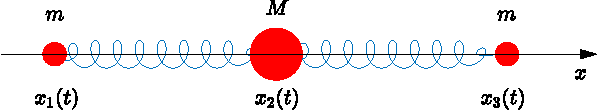
\includegraphics[width=8cm]{images/linear_water.pdf}}
Let $x_1$ and $x_3$ be the displacement of the hydrogen atoms from their equilibrium positions, and  $x_2$ be the displacment of the oxygen molecule.
\vfill Treat the atoms as if they are connected by springs with stiffness $k$.
\vfill
From Newton's 2nd law:

\twomini[.3]{.45}{.65}{\vspace{-.5em}\algn{mx_1\pp &= k(x_2-x_1)\\
Mx_2\pp &= k(x_3-x_2)-k(x_2-x_1)\\
mx_3\pp &=- k(x_3-x_2)}\student{Let $\vec{x}= \mat{ccc}{x_1&x_2&x_3}^T\\$}
}{
\student{Then we have \algn{ \ddn{}{t}{2} \vec{x} &= \omega_0^2\mat{ccc}{-1&1&0\\\alpha&-2\alpha&\alpha\\0&1&-1}  \vec{x}\\  \\ w_0&=\sqrt{k/m} \qquad \alpha=m/M}}
}
}
\slide[The eigensolutions of our water model]{\vspace{-2em}
\[\ddn{}{t}{2} \vec{x} =\mathbf{A}\vec{x},\qquad \mathbf{A}=\omega_0^2\mat{ccc}{-1&1&0\\\alpha&-2\alpha&\alpha\\0&1&-1} \qquad \larray{w_0=\sqrt{k/m} \\ \alpha=m/M}\]
\student{
\algn{\lambda_1 &= -\omega_0^2 \qquad \qquad \quad \vec{v}_1 = \mat{ccc}{-1&0&1}^T \\
&\vec{x}_1 = \paren{c_1\cos(\omega_0 t) + c_2\sin(\omega_0 t) }\vec{v}_1\\\\
\lambda_2 &= 0 \qquad\qquad \qquad \quad \vec{v}_2 = \mat{ccc}{1&1&1}^T\\
&\vec{x}_2 = (c_3+c_4t) \vec{v}_2\\\\
\lambda_3 &=  -(1+2\alpha)\omega_0^2 \qquad \quad \vec{v}_3 = \mat{ccc}{1&-2\alpha&1}^T\\
&\vec{x}_3 = \paren{c_4\cos(\sqrt{1+2\alpha}\omega_0 t) + c_5\sin(\sqrt{1+2\alpha}\omega_0 t) }\vec{v}_3
}
}
}

\settoggle{covered}{false}

\slide[Eigenmode 1 ($\lambda=-\omega_0^2$)]{
\[\vec{x}_1 = \paren{c_1\cos(\omega_0 t) + c_2\sin(\omega_0 t) }\mat{c}{-1\\0\\1}\]\vfill
\centerline{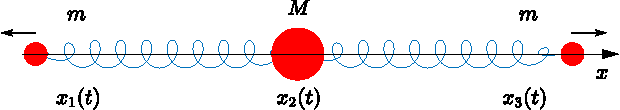
\includegraphics[width=10cm]{images/linear_water_emode1.pdf}}\vfill
\student{An oscillation with angular frequency $\omega_0$ where the middle atom remains fixed, and the outer atoms  move in opposite directions.}
\vfill
}

\slide[Eigenmode 2 ($\lambda=0$)]{
\twomini[.4]{.5}{.5}{\[\vec{x}_2 = \paren{c_3 + c_4 t }\mat{c}{1\\1\\1}\]}{\student{\algn{\text{Suppose } \vec{x}_2 &= T(t) \vec{v}_2\\
\ddn{}{t}{2}\vec{x_2} &= \mathbf{A}\vec{x}_2 = \lambda \vec{x}_2=\vec{0}=T\pp\vec{v}_2\\
T\pp&=0\\
\Rightarrow T(t) &= \text{linear function}}}}\vfill
\centerline{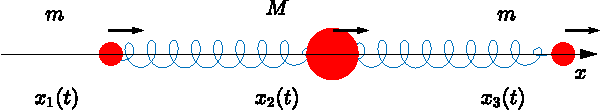
\includegraphics[width=10cm]{images/linear_water_emode2.pdf}}\vfill
\student{A translation of the whole molecule.}
\vfill
}

\slide[Eigenmode 3 ($\lambda=-(1+2\alpha)\omega_0^2$)]{
\[\vec{x}_3 =\paren{c_4\cos(\sqrt{1+2\alpha}\omega_0 t) + c_5\sin(\sqrt{1+2\alpha}\omega_0 t) }\mat{c}{1\\-2\alpha\\1}\]\vfill
\centerline{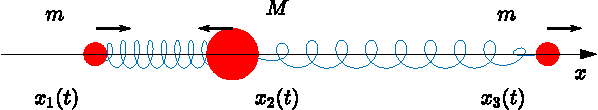
\includegraphics[width=10cm]{images/linear_water_emode3.pdf}}\vfill
\student{An oscillation with angular frequency $\sqrt{1+2\alpha}\omega_0$ where the middle atom  moves in the opposite directions as the two outer atoms.}
\vfill
}

\slide[A perturbation]{
Suppose we displace the leftmost hydrogen a distance $d$ and release it with zero velocity.\vfill
\centerline{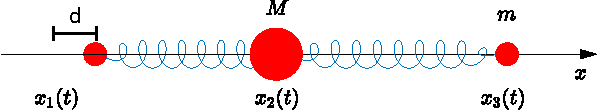
\includegraphics[width=10cm]{images/linear_water_displaced_hydrogen.pdf}}\vfill
That is, $\vec{x}(0)=\mat{c}{d\\0\\0}$ and $\vec{x}\p(0)=\vec{0}$\vfill

How will the system react?  \hfill - \hfill \small \href{https://www.desmos.com/calculator/ypd58rkmjc}{[Desmos Demo]}

}

\slide[]{
Notes:
\vfill
\student{The equations of motion of each atom can be decomposed into contributions from the three eigenmodes.

\vfill

How much each mode contributes is entirely determined by the initial conditions.

}
}
\slide[Now with forcing...]{
Suppose that  instead of moving the hydrogen atom, we apply a periodic force to it.
\[\ddn{}{t}{2} \vec{x} = \mathbf{A} \vec{x} + \mat{c}{d\\0\\0}\sin(\Omega t)\]
\student{
Method of undetermined coefficients
\[\vec{x}_p =  \cancelto{\vec{0}}{\vec{f}} \cos(\Omega t) + \vec{g}  \sin(\Omega t)\]\vfill
This assumes we have no resonance, i.e.
\[\Omega \neq \omega_0, 0, \sqrt{1+2\alpha}\omega_0\]
}
}


\slide{

\[\ddn{}{t}{2} \vec{x}_p = \mathbf{A} \vec{x}_p + \mat{c}{d\\0\\0}\sin(\Omega t)  \]\vfill
\[ \vec{x}_p = \vec{g} \sin(\Omega t) \qquad  \student{\Rightarrow \ddn{}{t}{2} \vec{x}_p  = -\Omega^2 \sin(\Omega t) \vec{g} } \]
\student{\algn{ -\Omega^2 \sin(\Omega t) \vec{g} & = \mathbf{A}\vec{g} \sin(\Omega t) +  \mat{c}{d\\0\\0}\sin(\Omega t) \\
-(\mathbf{A}+\Omega^2 \mathbf{I} ) \vec{g} &=  \mat{c}{d\\0\\0} \\ \vec{g} & = -(\mathbf{A}+\Omega^2 \mathbf{I} )^{-1} \mat{c}{d\\0\\0}  } }

}

\slide[Resonance]{\vspace{-2em}
\[\vec{x}(t) = \vec{x}_h(t)   -(\mathbf{A}+\Omega^2 \mathbf{I} )^{-1} \mat{c}{d\\0\\0} \sin(\Omega t) \]

Does the matrix $ (\mathbf{A}+\Omega^2 \mathbf{I} )^{-1} $ always exist?\vfill
\student{
No, not when $-\Omega^2$ is an eigenvalue of $\mathbf{A}$.\vfill Recall, to find the eigenvalue $\lambda$: \[\det(\mathbf{A}-\lambda \mathbf{I}) =0\]
Since, a matrix inverse has the $1/det$ in it, the matrix inverse would not exist.\vfill

This corresponds to resonance.
}\vfill
}
\slide[Resonance Demo]{
\[\ddn{}{t}{2} \vec{x} = \omega_0^2\mat{ccc}{-1&1&0\\\alpha&-2\alpha&\alpha\\0&1&-1}  \vec{x} + \mat{c}{d\\0\\0}\sin(\Omega t) \quad \larray{w_0=\sqrt{k/m} \\ \alpha=m/M}\]\vfill
With $\alpha=0.5$, $\omega_0=0.1$ we have resonances at \algn{\Omega=\sqrt{-\lambda}&=\omega_0, \;0, \sqrt{1+2\alpha}\omega_0\\
&=0.1,\;0, \;0.141421}
\vfill

\href{https://www.desmos.com/calculator/n872rce1re}{[Desmos Demo]}
}

\end{document}